The electronic noise of the sensor is estimated through runs acquired
with the sensor in complete dark ({\it pedestal} runs). For each
pixel, the pedestal is computed as the average of the counts over many
events, while the electronic noise is computed as the root-mean-square
(RMS) of the counts. The distribution of the pixels RMS is shown in
Fig.~\ref{fig:noise}. The mode of the distribution is about 1.8
photons per pixels, but a tail is observed, with pixels having a
single-pixel noise of more than 5 photons per pixels.
The pedestal $\mu_i$ is then subtracted to the image pixel-by-pixel,
and a first noise suppression is applied by neglecting pixels with a
count less than $1.3\times\textrm{RMS}_i$, where $i$ represents the
pixel (\textit{zero suppression}). 
%
\begin{figure}[ht]
  \centering
  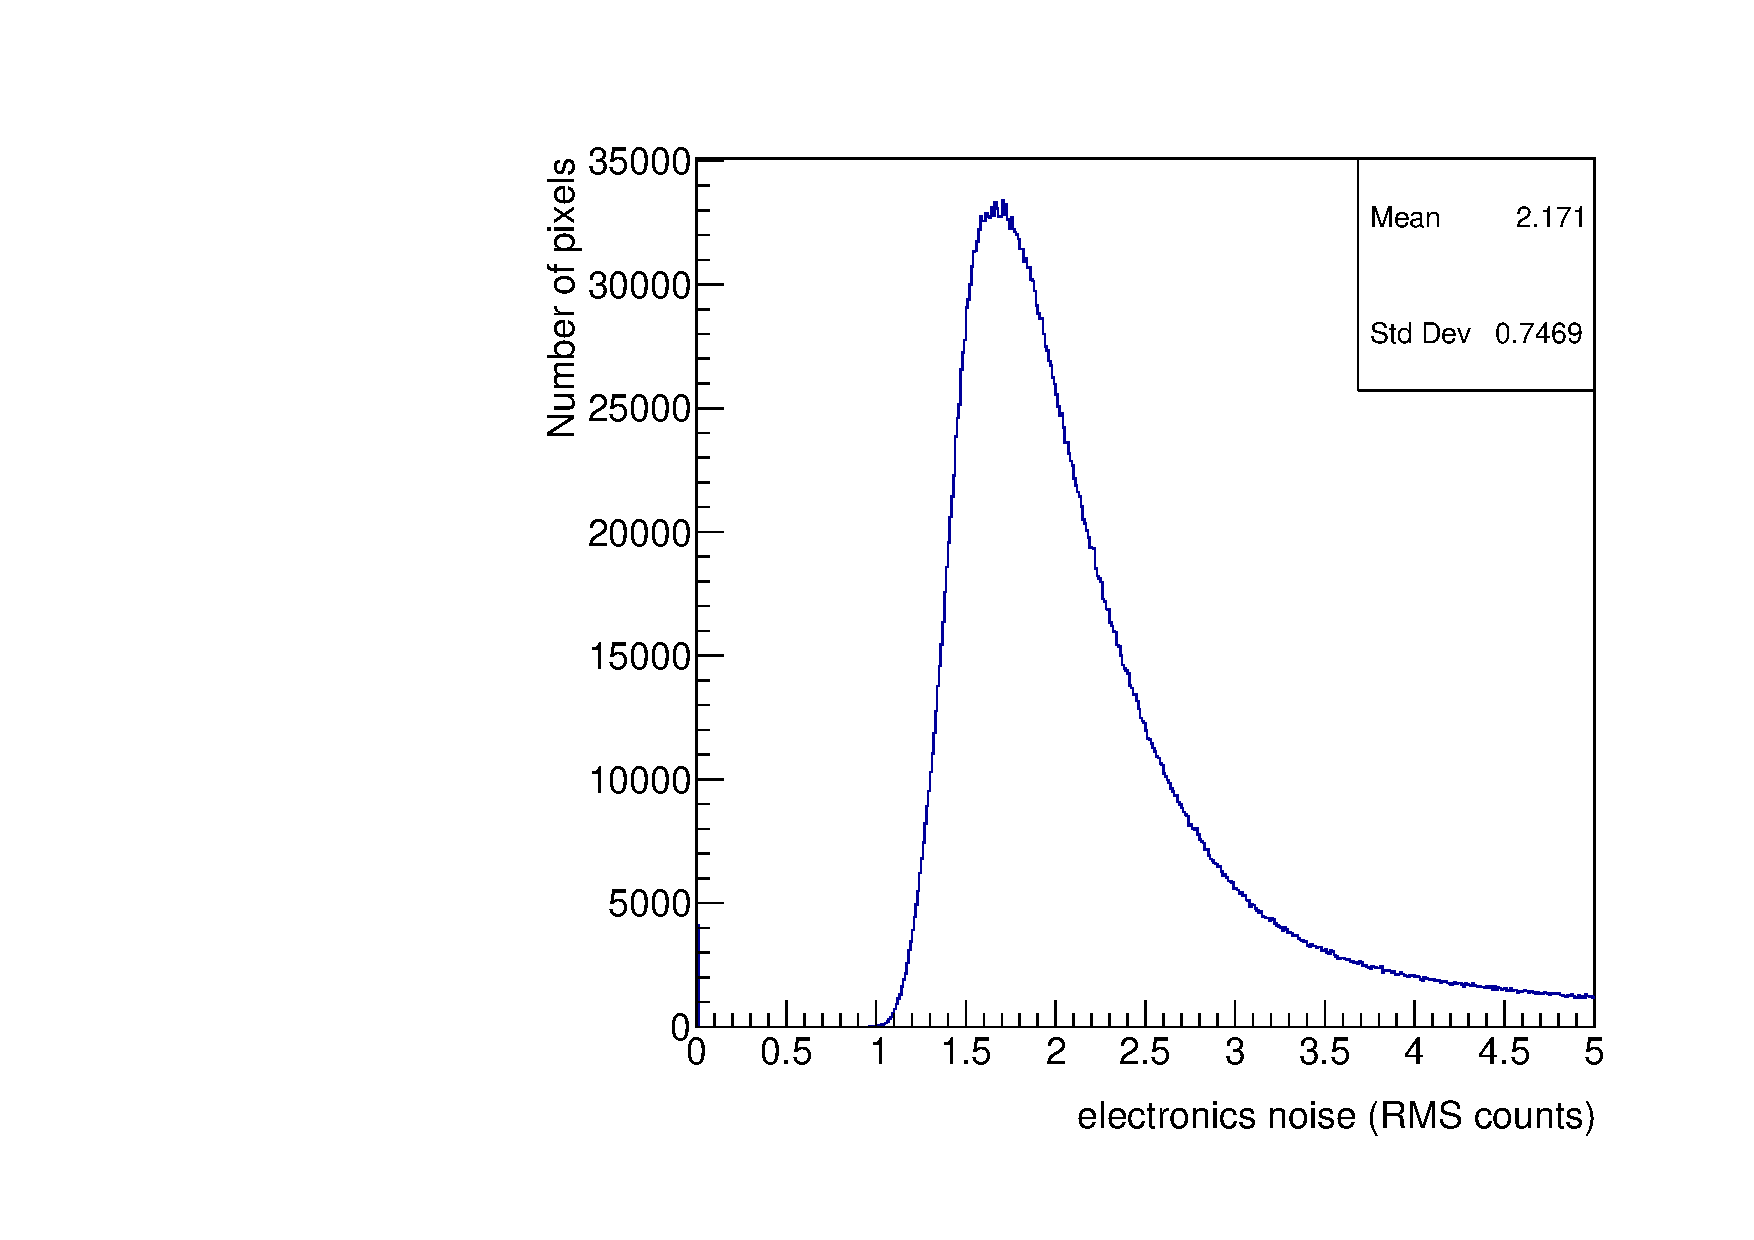
\includegraphics[width=0.45\linewidth]{figures/sensor_noise}
  \caption{Distribution of the electronic noise of the sensor,
    estimated in images taken with sensor in complete dark, and
    evaluated as the RMS of the distribution of the counts for each
    pixel.  \label{fig:noise}}
\end{figure}
%
On such pedestal-subtracted, zero-suppressed images, an upper
threshold is applied to reject hot pixels, which are more likely due
to sensor instabilities than to energy deposition. These are not
broken pixels, because they disappear in different places after a
power cycle of the camera, so a dynamic (run-by-run) suppression is
needed.  They are efficiently identified as high-intensity, isolated
pixels, and distinguished by a true energy deposit, for which each
pixel is surrounded by some other active pixel. A minimum average of
the counts, and a minimum number of two pixels above noise in a
$3\times3$ pixels matrix surrounding the hot pixel is required.

The resolution of the resulting image is then reduced by creating
\textit{macro-pixels}, by averaging the counts in $4\times4$ pixels
matrices. This is needed to reduce the combinatorics of the following
clustering algorithms, in order to run in a reasonable time for each
image. On such $512\times512$ pixels map, a median
filtering~\cite{medianfilter} is applied, as described in more details
in Ref.~\cite{medianfilter_cygno}. The output image is passed to the
basic clustering algorithm, described in the following.


